\chapter{Конструкторская часть}
\section{Схемы алгоритмов}

Ниже приведены схемы алгоритмов, упомянутых в аналитической части:
\begin{itemize}
	\item на рисунке~\ref{fig:complete_scheme} --- схема полного перебора для поиска гамильтонова пути;
	\item на рисунке~\ref{fig:aco_scheme} --- схема муравьиного алгоритма.
\end{itemize}
\begin{figure}[H]
	\centering
	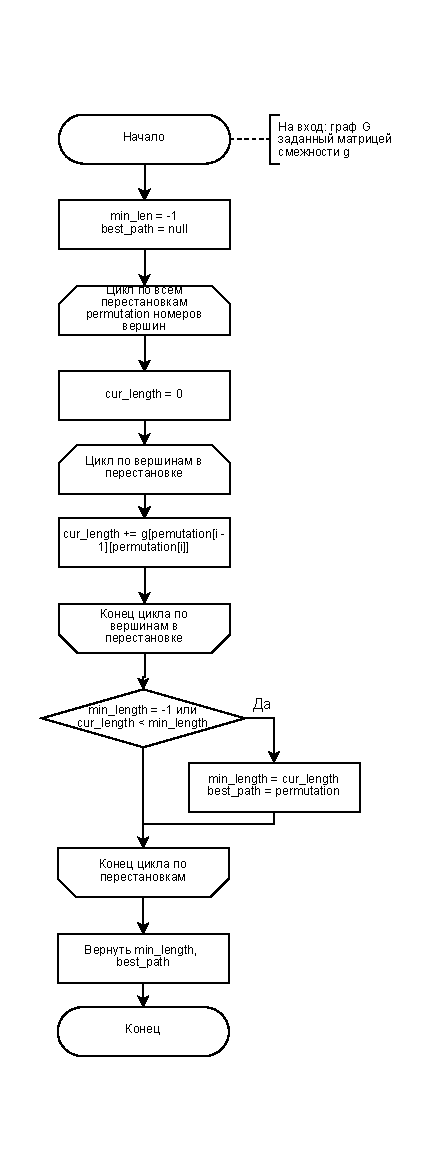
\includegraphics[width=0.5\textwidth]{complete_burst.pdf}
	\caption{Схема алгоритма полного перебора}
	\label{fig:complete_scheme}
\end{figure}
\begin{figure}[H]
	\centering
	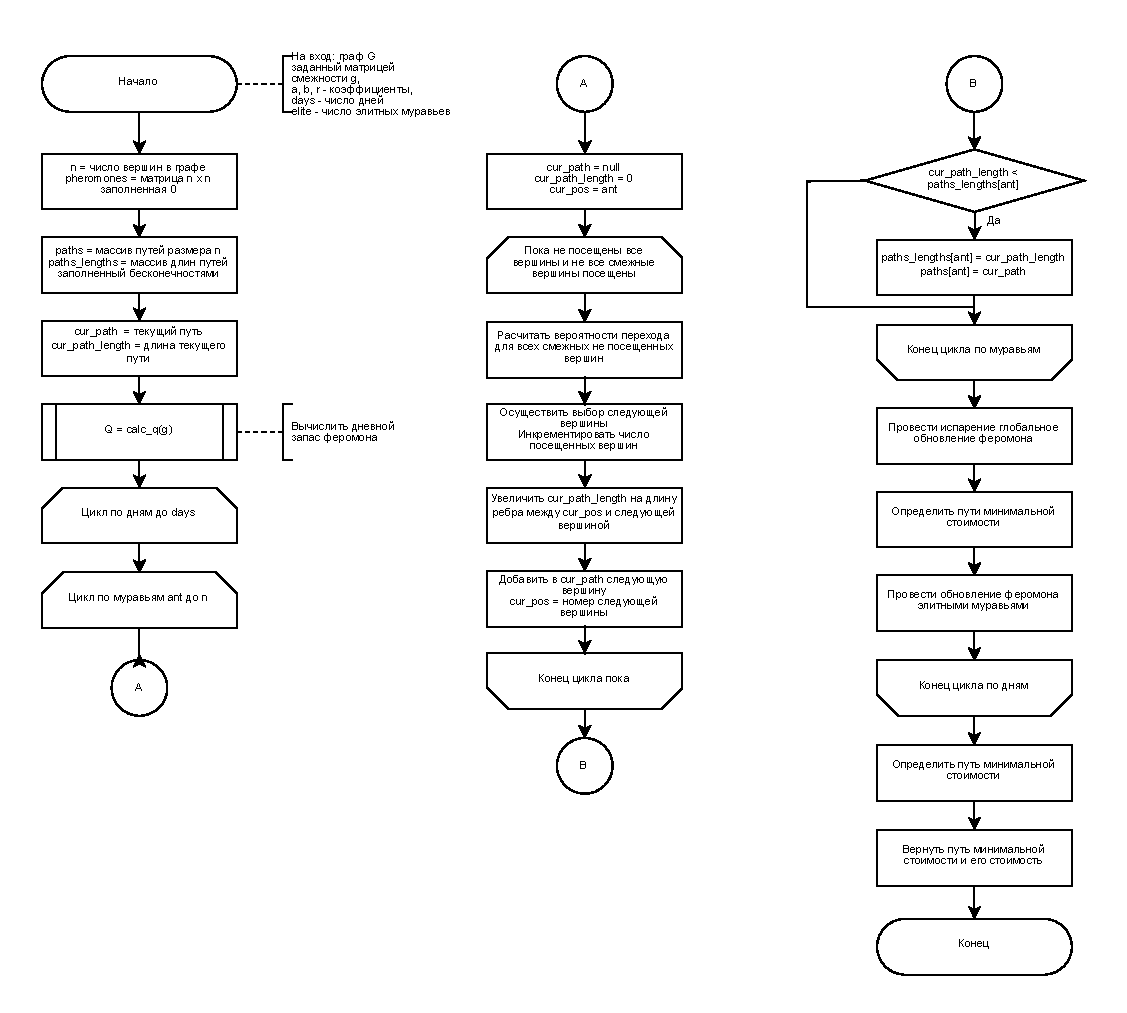
\includegraphics[width=\textwidth]{ACO.pdf}
	\caption{Схема муравьиного алгоритма}
	\label{fig:aco_scheme}
\end{figure}
\section*{Вывод}

На основе аналитической части построены схемы алгоритмов решения задачи коммивояжера.

\clearpage